\documentclass[tikz]{standalone}
\usepackage{pgfplots}
\usepackage{mathptmx}
\usepackage{ctex}
% \pgfplotsset{compat=1.16}
\begin{document}
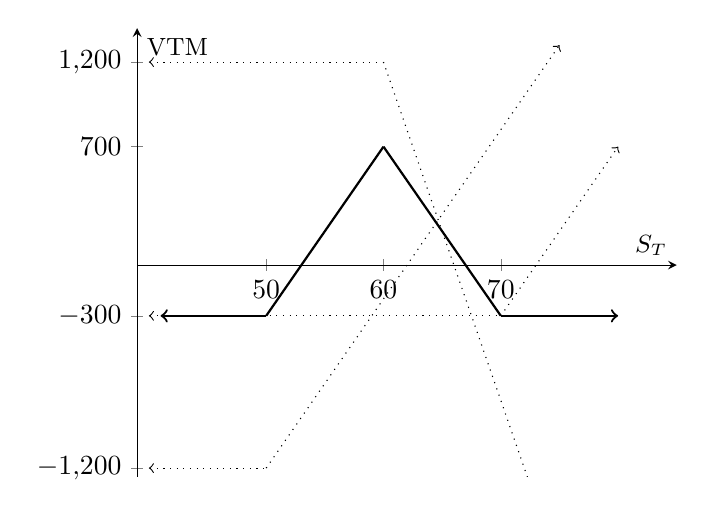
\begin{tikzpicture}
    \begin{axis}[
        axis lines = middle,
        xlabel = {$S_T$},
        ylabel = {VTM},
        ymin=-1250, ymax=1400,
        xmin=39, xmax=85,
        xtick={50,60,70},
        ytick={-1200,-300,0,700,1200},
        % width=10cm,
        % height=7cm,
        % axis equal,
        label style={font=\small}
    ]
    % 定义参数
    \def\Ka{50} % 执行价格
    \def\Kb{60} % 执行价格
    \def\Kc{70} % 执行价格
    \def\Pa{12}  % 期权费
    \def\Pb{6}  % 期权费
    \def\Pc{3}  % 期权费
    
    % 绘制看涨期权到期收益曲线
    \addplot[domain=40:\Ka,<-,dotted] {(-\Pa)*100};
    \addplot[domain=\Ka:75,->,dotted] {(x-\Ka-\Pa)*100};

    \addplot[domain=40:\Kc,<-,dotted] {(-\Pc)*100};
    \addplot[domain=\Kc:80,->,dotted] {(x-\Kc-\Pc)*100};

    \addplot[domain=40:\Kb,<-,dotted] {2*\Pb*100};
    \addplot[domain=\Kb:75,->,dotted] {(\Kb-x+\Pb)*2*100};
    
    \addplot[domain=41:\Ka,<-,thick] {-300};
    \addplot[domain=\Ka:\Kb,thick] {(x-53)*100};
    \addplot[domain=\Kb:\Kc,thick] {(67-x)*100};
    \addplot[domain=\Kc:80,->,thick] {-300};
    \end{axis}
\end{tikzpicture}

\end{document}